\section{Lattice matrix elements and simulation setup}\label{sec:setup}
%{\it Numerical setup:}\ 

The standard non-perturbative renormalization of lattice matrix elements is through 
calculating some auxiliary matrix elements of the operator (which can also be computed in perturbation theory) and using them as the 
renormalization factor to approach the continuum limit. 
In this paper, we focus on the study of the auxiliary matrix elements 
potentially useful for the renormalization of quasi-LF correlations. We
mainly consider the matrix elements of the quasi-PDF operators in the 
following cases: 1) in a large Euclidean momentum quark state, 2) in the
physical zero-momentum state of a hadron such as the pion or nucleon.
We will also study the matrix element in the vacuum~\cite{Braun:2018brg} (case 3), and show that it is not a good choice for renormalization because at small $z$ such a  matrix element is suppressed as can be shown by operator
product expansion (OPE). 
Moreover, since the $z$-dependent renormalization is mainly associated 
with the Wilson link, we shall also consider the matrix elements of Wilson loop as well as the Wilson link in a fixed gauge (case 4).  

We calculate the pion and nucleon matrix elements $\tilde{h}^{0}_{H}(z)=\langle H| O_{\gamma_t}(z)|H \rangle_{\vec{P}=0}$ in the rest frame evaluating the following three-point function,
\begin{align}\label{eq:hadron}
&R_{H}(t_2,t,z)\equiv\frac{\langle O_H(t_2)\sum_{\vec{x}}O_{\gamma_t}(z;(\vec{x},t))O_H^{\dagger}(0)\rangle}{\langle O_H(t_2)O_H^{\dagger}(0)\rangle}\nonumber\\
&=\langle H| O_{\gamma_t}(z)|H \rangle\nonumber\\
&+{\cal O}(e^{-\delta m t})+{\cal O}(e^{-\delta m (t_2-t)})+{\cal O}(e^{-\delta m t_2}),
\end{align}
where $O_{\gamma_t}(z,(\vec{x},t))=\bar{\psi}(\vec{x},t) \gamma_t U((\vec{x},t),(\vec{x}+\hat{n}_z z,t)) \psi (\vec{x}+\hat{n}_z z,t)$, $\hat{n}_z$ is the unitary vector along the $z$ direction, and $O_H$ is the interpolation field of a hadron such as a pion and a nucleon.  $t_2$ corresponds to the source-sink separation. 

To obtain $\tilde{h}^0_{H}(z)$ accurately, we need both $t$ and $t_2-t$ to be large enough to suppress excited-state contaminations, or fit the three point function with a proper parametrization on the excited-state contaminations. We can use the first strategy for the pion case since the signal-to-noise ratio will not decay for the pion in the rest frame; while the second strategy is essential for the other cases where the statistical uncertainty increases exponentially with $t$ and $t_2$. Due to (anti)periodic boundary conditions we can use at most $t_2=T/2$ which is larger than 2 fm on most modern lattice ensembles. Since the mass gap $\delta m\sim $ 1 GeV between the ground and first exited state of pion  $\langle \tilde{h}^0_{\pi}(z)\rangle$ can be extracted with sufficient  accuracy. At small perturbative $z$, $\langle \tilde{h}^0_{\pi}(z)\rangle^{-1}$ acts as a renormalization factor up to certain ${\cal O}(\Lambda_{\rm QCD}^2z^2)$ power corrections~\cite{Orginos:2017kos}.

A common non-perturbative renormalization method for lattice QCD matrix elements with local operators is the RI/MOM scheme~\cite{Martinelli:1994ty} and its modified versions~\cite{Aoki:2007xm}. One can calculate the bare matrix element with given operators in an off-shell quark state, for both the lattice and dimensional regularizations, and renormalize their difference in the $\overline{\textrm{MS}}$ scheme to get the renormalization factor for the bare quantities. For the quasi-PDF, such a renormalization constant (the RI/MOM renormalization factor) is defined through the $O_{\gamma_t}(z)$ matrix element in the off-shell quark state with given momentum $p^2$~\cite{Green:2017xeu,Chen:2017mzz,Alexandrou:2017huk,Stewart:2017tvs}:
\begin{align}\label{eq:Z_ri}
&Z^{RI}(z,\mu_R)=\frac{1}{4N_c}\textrm{Tr}[\gamma_t\langle q|O_{\gamma^t}(z)|q\rangle]|_{p^2=-\mu_R^2,p_z=p_t=0},
\end{align}
where $N_c=3$ is the number of colors, $\mu_R$ is the RI/MOM renormalization scale. We will take $\mu_R$ = 3 GeV since the RI/MOM factor has little dependence on the renormalizaiton scale in a certain range~\cite{Zhang:2020rsx}. We work with Landau gauge fixed configurations, and choose $p_z=p_t=0$ to eliminate the difference between the projections~\cite{Liu:2018uuj}. 
%We also 
%analyze the $O_{\gamma_t}(z)$ matrix element in the off-shell quark state directly.

Factor $Z^{RI}$ can be calculated non-perturbatively for any lattice regularization, or equivalently for any quark and gluon action defined on the lattice. However, the current lattice QCD calculation is limited to the Landau gauge. The perturbative matching with off-shell states in Landau gauge can be complicated beyond one-loop level~\cite{Chen:2020ody}. 


The $z$-dependent part of renormalization comes from the Wilson line, therefore 
one may extract the linear divergences from matrix elements of pure Wilson lines.
First one can consider a Wilson loop~\cite{Chen:2016fxx,Zhang:2017bzy,Musch:2010ka,Green:2017xeu,Chen:2017gck},
\begin{equation}
{\cal U}(r,t)=\langle U(\vec{r},t;\vec{r},0)U(\vec{r},0;\vec{0},0)U(\vec{0},0;\vec{0},t)U(\vec{0},t;\vec{r},t)\rangle , 
\end{equation}
Ref.~\cite{Chen:2016fxx} proposed this scheme to renormalize the pion DA, and the linear divergence coefficient was extracted precisely based on the calculation with several lattice spacings  in the following Kaon DA study~\cite{Zhang:2017bzy}. But most of subsequent lattice QCD calculations have switched to the RI/MOM scheme or used a hadronic matrix element.

 One can also consider the matrix element of a single Wilson Link $\langle U(0,z)\rangle$ in a fixed gauge such as the Landau gauge. As the simplest choice without any external state, $\langle U(0,z)\rangle$ can provide a reference to identify whether the linearly divergent behavior is sensitive to the existence of the external state, as suggested in the multiplicative renormalizability studies of the quasi-PDF operator~\cite{Ji:2015jwa, Ji:2017oey,Ishikawa:2017faj,Green:2017xeu}.
 
\begin{table}[htbp]
  \centering
  \begin{tabular}{c|ccrc}
  \toprule
 symbol & $6/g^2$ & $L$ & $T$  & $a(\mathrm{fm})$ \\
\hline
a12m310 &  3.60 & 24 & 64  & 0.1213(9) \\
\hline
a09m310 &  3.78 & 32 & 96 & 0.0882(8)  \\
\hline
a06m310 &  4.03 & 48 & 144 & 0.0574(5) \\
\hline
a04m310 &  4.20 & 64 & 192 & 0.0425(4)  \\
\hline
a03m310 &  4.37 & 96 & 288 & 0.0318(3) \\
\hline
  \end{tabular}
  \caption{Setup of the MILC ensembles, including the bare coupling constant $g$, lattice size $L^3\times T$, and lattice spacing $a$.}
  \label{tab:lattice}
\end{table}

\begin{table}[htbp]
  \centering
  \begin{tabular}{c|ccrccc}
  \toprule
 symbol & $6/g^2$ & $L$ & $T$ &  $a(\mathrm{fm})$\\
\hline
DW11 & 2.13 &24 & 64  & 0.1105(3) \\
\hline
DW08 & 2.25 &32 & 64  & 0.0828(3) \\
\hline
DW06 & 2.37 &32 & 64  & 0.0627(3) \\
\hline
  \end{tabular}
  \caption{Setup of the RBC ensembles, including the bare coupling constant $g$, lattice size $L^3\times T$, and lattice spacing $a$.}
  \label{tab:lattice2}
\end{table}

%{\color{blue}Following two sections need be reworked by lattice guys....}
  
Our lattice calculations are performed using the Chroma software suite~\cite{Edwards:2004sx} and QUDA~\cite{Clark:2009wm,Babich:2011np,Clark:2016rdz} in the HIP programming model~\cite{Bi:2020wpt}. We use 2+1+1 flavors (degenerate up and down, strange, and charm degrees of freedom) of highly improved staggered quarks (HISQ)~\cite{Follana:2006rc} ensembles generated by the MILC Collaboration~\cite{Bazavov:2012xda} at five lattice spacings, and 2+1 
flavor domain wall (DW) quarks and Iwasaki gauge
ensembles from the RBC/UKQCD collaboration~\cite{Blum:2014tka} at
three lattice spacings. The pion mass for all ensembles are tuned to be roughly 310 MeV based on the pion mass of the light sea quark mass on the corresponding ensemble. The lattice spacings for the MILC ensembles are determined using Wilson flow based on the parameters determined by Ref.~\cite{Miller:2020evg}.

We use the matrix elements without hyper-cubic (HYP) smearing in order
to test the perturbative renormalization analysis (Sec.~\ref{sec:test},~\ref{sec:StrtoRe}, and~\ref{sec:highorder}). 
However, since in practical calculations the results without smearing can 
be rather noisy, it is standard to use some type of smearing in lattice simulations. It is unclear to us how strongly the smearing will interfere with renormalization. Therefore, we regard our method as a purely phenomenological approach for the time being to analyze data with one step HYP smearing~\cite{Hasenfratz:2001hp} in Sec.~\ref{sec:smearing} and~\ref{sec:otherresult}, hoping that the gain in statistical precision outweighs the additional systematic uncertainty 
from moderate smearing.


We use two kinds of fermion actions for the valence quarks: clover and overlap fermions. Clover fermions break chiral symmetry and the action is defined by
\begin{align}\label{eq:clover}
S^{clv}_{q}=&\sum_{x}\bar{\psi}(x)\bigg[\frac{1-\gamma_{\mu}}{2a}U_{\mu}(x,x+\hat{n}_{\mu})\psi(x+\hat{n}_{\mu})\nonumber\\
&+\frac{1+\gamma_{\mu}}{2a}U_{\mu}(x,x-\hat{n}_{\mu})\psi(x-\hat{n}_{\mu})\nonumber\\
&-\left(\frac{4}{a}+c_{sw}\sigma_{\mu\nu} F_{\mu\nu}(x)a+m_q^0\right)\psi(x)\bigg],
\end{align}
where $\hat{n}_{\mu}$ is the unit vector along the $\mu$ direction, the clover coefficient $c_{sw}$ is the tadpole improved tree level value, and $m^0_{q}a$ is the bare quark mass which is determined by requiring the pion mass to be roughly 310 MeV.  Parameters $c_{sw}$ and $m^0_{q}a$ should approach 1 and 0 respectively in the continuum, while the lattice spacing dependence is weaker than the ${\cal O}(a)$ discretization effect in the present range of $a$, and closer to that of the gauge coupling $g^2$ as predicted by lattice perturbative theory. 

The overlap action preserves chiral symmetry but the simulation is rather expensive. We use it to test
the dependence of renormalization on the fermion action. 
The overlap fermion action is defined by~\cite{Chiu:1998eu, Liu:2002qu} 
\begin{align}
S^{\textrm{ov}}_{q}&=\sum_{x,y}\bar{\psi}(x) D_{\textrm{ov}}(x,y)\psi(y),\\
 D_{\textrm{ov}}&=\rho\Big(1+\frac{D_\textrm{w}(-\rho)}{\sqrt{D^{\dagger}_\textrm{w}(-\rho)D_\textrm{w}(-\rho)}}\Big),\nonumber
\end{align}
where
\bea
&D_\textrm{w}(m^{\textrm{w}}_q;x,y)=\frac{1-\gamma_{\mu}}{2a}U(x,x+\hat{n}_{\mu})\delta_{x+\hat{n}_{\mu},y}\nonumber\\
&+\frac{1+\gamma_{\mu}}{2a}U(x,x-\hat{n}_{\mu})\delta_{x-\hat{n}_{\mu},y}-(\frac{4}{a}+m^{\textrm{w}}_q)\delta_{x,y},
\eeq
and $-\rho$ should be smaller than the bare quark mass for which vanishes the pion mass to make $D_{\textrm{ov}}$ to be the same as the standard Dirac operator in the continuum limit. We choose $-\rho=1.5$.

Although different active and sea fermion formulations
will in general introduce non-unitarity, the effect
shall vanish in the continuum limit. However, at finite $a$,
the difference will generate systematic uncertainties 
which can affect the final results. 

 \begin{figure}[tbp]
  \centering
  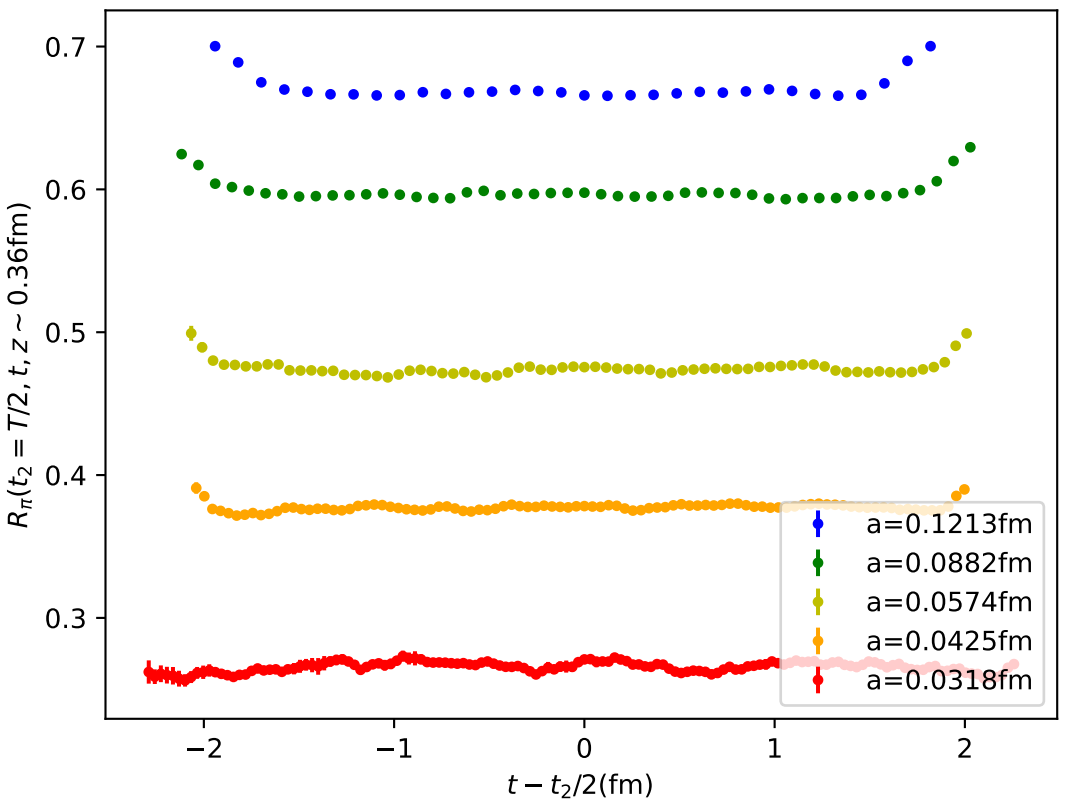
\includegraphics[width=8cm]{images/ME_pion.png}
   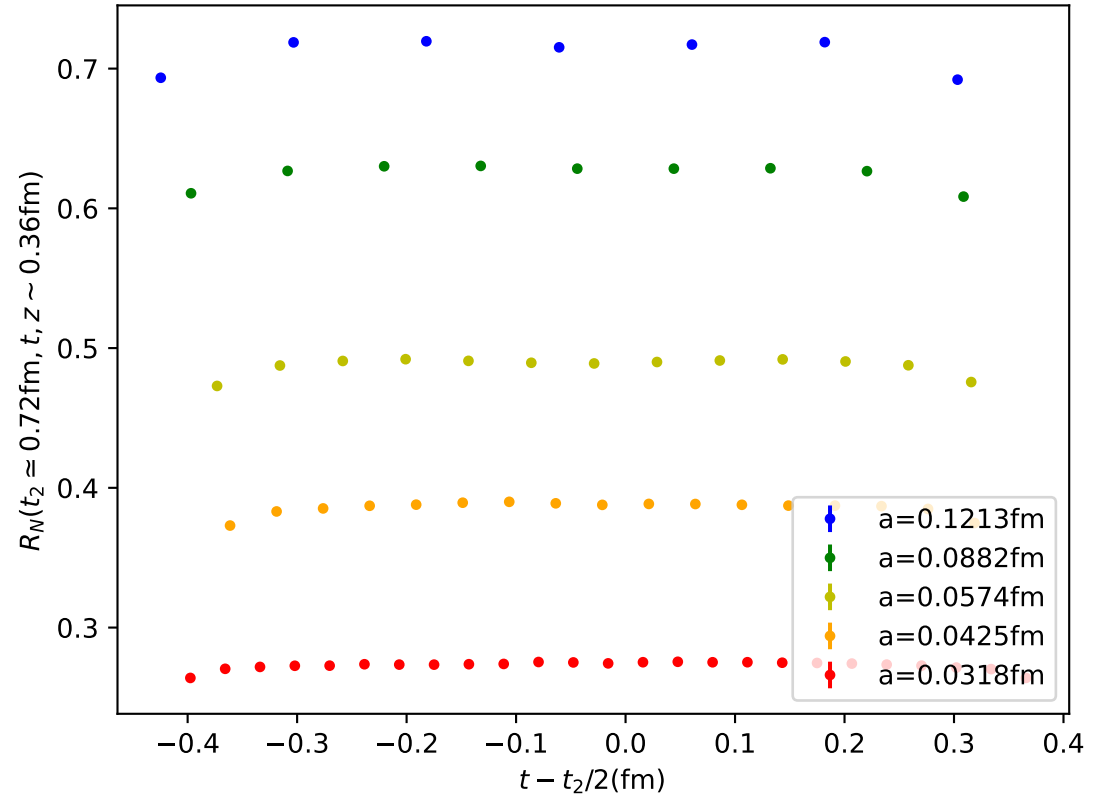
\includegraphics[width=8cm]{images/ME_nuc.png}
  \caption{The bare ratio $R_{\pi}(t_2=T/2,t,z)$ for the pion (upper panel) and $R_{N}(t_2\simeq 0.72 \textrm{fm},t,z)$ for the nucleon (lower panel) with $z\sim$ 0.36 fm. For the pion case, we can see that the data in the region between $t-t_2/2\in[-1,1]$ fm are consistent with each other up to statistical fluctuations. For the nucleon case the ratio is also flat around $t\sim t_2/2$.}
  \label{fig:pion_plateau}
  \end{figure}

We start with nucleon and pion matrix elements for the MILC ensembles and clover action. For the pion matrix element, We average the $R_{\pi}(t_2,t,z)$ data with $t_2=T/2$ and $t\in[T/8,3T/8]$ to get a precise estimate of the ground state matrix element, and it should be also precise since $T$ is between 7.7 and 9.1 fm in the ensembles we used, as shown in the upper panel of Fig.~\ref{fig:pion_plateau}. Note that $R_{\pi}(T/2,T/4,z)$ equals to $\langle \pi| O_{\gamma_t}(z)|\pi \rangle/2$ in such a case. The additional factor 1/2 corrects for the fact that there are forward and backward propagating states for (anti)periodic boundary conditions. The nucleon case is known to be much noisier especially at large $t_2$. Thus, we just consider $t_2=2t\simeq 0.72$ fm in all cases, and plot $R_{N}(t_2,t,z)$ in the lower panel of Fig.~\ref{fig:pion_plateau}.

 \begin{figure}[tbp]
  \centering
  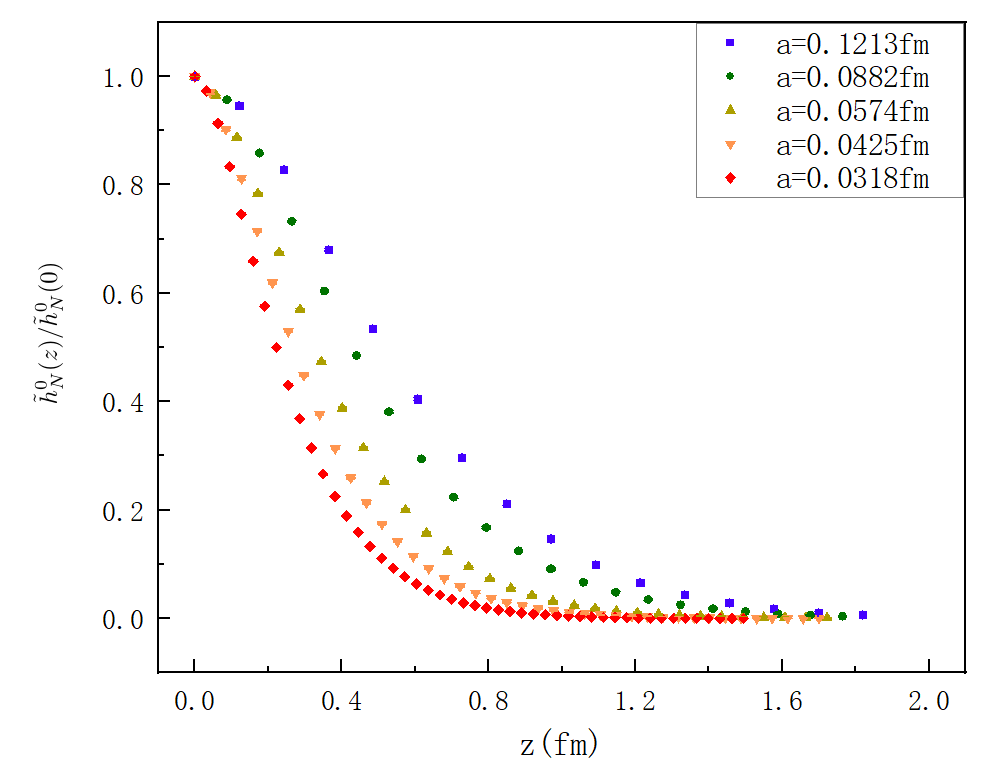
\includegraphics[width=8.5cm]{images/h_nuc_bare.png}
  \caption{The normalized bare nucleon matrix element in the rest frame, $\tilde{h}^0_{N}(z)/\tilde{h}^0_{N}(0)$ as the function of the Wilson link length $z$. The matrix element has a fast exponential decay at large $z$ and the decay process accelerates with smaller
  lattice spacings.}
  \label{fig:ratio_had}
  \end{figure}

The normalized bare $\tilde{h}^0_{N}(z)/\tilde{h}^0_{N}(0)$ where $\tilde{h}^0_{N}(z)$ is approximated by $R_{N}(t_2,t,z)$ with $t_2=2t\simeq 0.72$ fm is plotted in Fig.~\ref{fig:ratio_had}, with a normalization factor $1/\tilde{h}^0_{N}(0)$ using jackknife resampling to make it to be exactly one at $z=0$ at all lattice spacings. As in the figure, the linear divergence makes $\tilde{h}^0_{N}(z)/\tilde{h}^0_{N}(0)$ decay exponentially with both $z$ and $a$, and thus one cannot obtain any meaningful continuum limit when $a\to 0$. A renormalization is necessary to recover a good continuum limit.
